\fancyhead[LO]{{\scriptsize {\FA \ }我们最幸福 {\FA } 手风琴与黑板}}%奇數頁眉的左邊
\fancyhead[RO]{{\tiny{\textcolor{Gray}{\FA \ }}}\thepage}
\fancyhead[LE]{{\tiny{\textcolor{Gray}{\FA \ }}}\thepage}
\fancyhead[RE]{{\scriptsize {\FA \ }我们最幸福 {\FA } 手风琴与黑板}}%偶數頁眉的右邊
\fancyfoot[LE,RO]{}
\fancyfoot[LO,CE]{}
\fancyfoot[CO,RE]{}
\chapter*{08 {\FA } 手风琴与黑板}
\addcontentsline{toc}{chapter}{\hspace{5mm}08 \textbf{>}\ \ 手风琴与黑板}
\begin{flushright}
	\textcolor{PinYinColor}{\EN \huge{The Accordion\\
		and the Blackboard\\
	\ \\}}
\end{flushright}
\begin{figure}[!htbp]
	\centering
	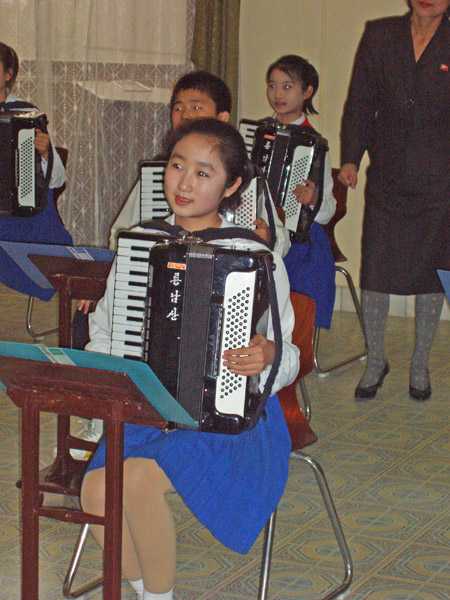
\includegraphics[width=6cm]{./Chapters/Images/08.jpg}
	\caption*{2005年平壤的手风琴课}
\end{figure}


金日成的逝世使得美兰最后一门音乐考试推迟,因此直到1994年秋天,她才得以毕业。考虑到金日成刚刚去世,因此在此时开始自己的教师生涯,可真不适时宜,对所有其它事情也一样。此时,美兰却很急切的想回到家里,和父母在一起,清津的食品供给已经完全中断了。她要求分配到离家较近的地方教学。幸运的是,最终她被派往位于她父亲曾经工作过的Saenggiryong矿附近的幼儿园当老师。矿场距离镜城3公里,在通往清津的主路上,位于奶咖啡色的山间。对于能够回来工作,美兰的父母也放心了些,这样她能吃的好一些。在北朝鲜,未结婚的子女,特别是女儿同父母住很平常。她能够帮这料理些家务,还可以陪陪父亲,那些日子他已经几乎不上班了。他们的口琴屋里的两个卧室由于两个大些的女儿已经出嫁,儿子考进师范学院,现在也显得空空荡荡。\\

从家到幼儿园大概步行需要45分钟,而且幼儿园看上去和她在清津实习的那个一模一样。那是个单层的混凝土建筑,要不是围着房子的铁栅栏上画满五颜六色的向日葵,入口处有个拱门上面写着“我们很幸福”谁也看不出这是个幼儿园。在门口的院子里,有几件破旧的运动设施──一个秋千,木质的座板早已破烂,一部滑梯,还有一个爬架。教室都是些标准的配备,黑板上挂着金日成父子画像。双人的课桌也是用木板和铁架做成的。在教室的一边,窗户下是迭起来的床垫,用于午睡。另外一边有个很大的书架,只有很少的几本书现在也几乎看不清了,这些书是很早以前的复印件,现在也是污迹斑斑了。书本和纸张在北朝鲜很珍贵,如果想让孩子们在家学习,那么一些有毅力的母亲就要去手抄课本。\\

学校之间的差别主要在于学生本身。乡村的孩子们看上去就比他们在城市的同龄人要穷很多。幼儿园期间还没有制服,因而孩子们穿的也都是五花八门,大多都是哥哥姐姐传下来的衣服。因为学校没有暖气,孩子们一个个都是裹的一层又一层的。有些孩子衣衫褴褛的都会让美兰惊讶,他们穿的破破烂烂。当美兰帮孩子们脱衣服的时候,她发现一层又一层的衣服下面,包裹着的是那么瘦小的身体。当美兰握着孩子们纤细的手时,孩子们的拳头在她的手掌里只有核桃大小。这些5-6岁大的孩子,怎么看都像只有3-4岁的样子。在清津实习的时候,她的学生大多是工厂工人或者当官人家的孩子;而这些都是矿工的孩子。美兰意识到,虽然城市里的食物供应很成问题,但是矿场食物短缺更严重。在过去,为了奖励他们的重体力劳动,矿工能得到每天900克的粮食配给,多过普通工人的700克。现在Saenggiryong附近的煤矿和高岭土矿差不多都关闭了1年多时间,矿工的粮食配给也早就中断了。美兰怀疑有些孩子来幼儿园仅仅是为了中午能吃上一顿餐厅提供的,一份和她大学时餐厅里一样的,只放点盐、飘着几片干菜叶的清汤。\\

虽然如此,美兰还是满怀热情的投入到新的工作当中。身为教师,是个受过教育,倍受尊重的阶层。这对于一个矿工的女儿还说是一个巨大的进步,再也不是身处社会的最低阶层了。每天早上她都迫不及待的起床,穿上在床底压了一宿的,爱起皱的白衬衣。\\

学校早8点上课。每当此时,美兰就会挂着灿烂的笑容去迎接孩子们,看着他们慢慢坐满教室。当她把孩子们一个个领到指定好的座位上,她就会拿出她的手风琴。在北朝鲜,每一个教师都要求会弹奏手风琴,这也是她毕业前的最后一项测试。手风琴也被称为“人民乐器”,因为当人们到建筑工地,或者在田间地头的义务劳动时很容易携带上它──也没有什么其它乐器能给田野里或者建筑工地上劳作的工人带来手风琴所能带来的巨大干劲。在课堂里,老师经常唱《这个世界我们无所羡慕》,在北朝鲜这就如《一闪一闪亮晶晶》一样,是家喻户晓的一首歌曲。\\

美兰还是小姑娘的时候,这些歌词就深深的印在心里:\\

\begin{quote}
	\begin{spacing}{1.0}  %行間距倍率
		\textit{{\footnotesize 	我们的父亲,这个世界我们无所羡慕。\\
		我们的家园在劳动党的怀抱之中。\\
		我们都是兄弟姐妹。\\
		即使面对火海,可爱的小朋友们请不用害怕。\\
		因为父亲在这里。\\
		这个世界,我们无所羡慕。\\}}
	\end{spacing}
\end{quote}

美兰没有像她姐姐那样的好嗓子──俊相曾经这样揶揄她,每次她唱歌的时候,俊相都是避而远之。可是她的小小学生没这么挑剔。当她唱的时候,他们都仰着小脸看着她,很是活泼可爱。孩子们都很崇拜她,这样也激起她的热情。美兰曾经很沮丧于自己的弟弟和自己年龄相仿,事事总是和他竞争,相比之下,她更喜欢教导这些小弟弟小妹妹们。她很喜欢她的工作,至于她教些什么,她不曾停下来想想是对是错。她也不知道教育可以会是其它的什么样子。\\

1977年,金日成在他的一篇关于社会主义教育的文章中这样写到,“只有在适当的政治意识形态的基础上,科学,技术以及体育教育才能得以成功。”由于美兰的学生还小,还读不了伟大领袖的通篇巨作\footnote{以金日成的名字出的书多达一打,而金正日也写了另外一打的书。},她只是大声的朗读着这些摘选。孩子们也被鼓励跟着她齐声朗诵关键篇章。一个可爱的小女孩或小男孩用孩子气的嗓音大声背诵金日成的语录总能引得大人们一片开心的笑声。在意识形态训练之后,接下来的课程就是一些比较普通的科目,但是伟大领袖总是形影相随。不论是学习数学、科学、阅读、音乐或者艺术,孩子们总被教导爱戴领袖,憎恨敌人。举个例子,一个1年级的数学书上是这样提问的:\\

\begin{quote}
	\begin{spacing}{1.0}  %行間距倍率
		{\footnotesize 	\textit{“八个男孩,九个女孩一起歌唱金日成赞歌。一共有多少个孩子在唱歌?”}\\

		\textit{“一个女孩在抗日战争中作为爱国军队的通信员。她把情报放在一个装有五个苹果的篮子里,但是在一个检查点,被一个日本兵拦住。这个日本兵拿走了两个苹果。现在篮子里还有几个苹果?”}\\

		\textit{“三个朝鲜人民军战士消灭了三十个美国大兵。如果这三个士兵每人消灭的美国大兵一样多,每个战士消灭多少个美国大兵?”}\\}
	\end{spacing}
\end{quote}

2003年出版的一本1年级的启蒙阅读材料里有这么一首诗,题目是“我们前往何方?”\\

\begin{quote}
	\begin{spacing}{1.0}  %行間距倍率
		\textit{{\footnotesize 	我们曾去过什么地方?\\
		我们曾到过森林。\\
		我们将去往何方?\\
		我们即将翻越山峦。\\
		我们将做什么?\\
		我们将去消灭日本鬼子。\\}}
	\end{spacing}
\end{quote}

音乐课上还教一首名为“朝美国混蛋开枪”的歌曲:\\

\begin{quote}
	\begin{spacing}{1.0}  %行間距倍率
		\textit{{\footnotesize 	我们的敌人就是美国混蛋\\
		他们想霸占我们美丽的祖国\\
		拿起我自己亲手做的枪\\
		我将朝他们开枪……\\}}
	\end{spacing}
\end{quote}

儿童启蒙读物里通篇都是孩子们被西方传教士、日本鬼子或者美帝国主义者殴打、刀刺、火烧、泼酸或者扔到水井里的故事。在一个广为流传的故事里,一个小男孩仅仅因为拒绝给美国大兵擦皮鞋就被一脚踢死了。同当年纳粹德国的反犹漫画里的犹太人一样,在北朝鲜,美国大兵都被画成有着一个鹰钩鼻。\\

美兰听过很多关于美国在朝鲜战争期间的暴行,但是她不知道哪些是不是真的。她自己的妈妈回忆那些曾经经过他们家乡的美国大兵时,说他们又高又帅。\\

“我们常常追在他们后面跑。”她妈妈回忆道。\\

“追着他们?你没有逃走?”\\

“没有,他们会给我们口香糖。”她妈妈告诉她。\\

“你是说他们没有杀掉你?”当听到她妈妈的故事的时候,美兰感到不可思议。在历史课上,孩子们曾经有个参观。所有规模大些的小学都特别设有一个专门用于讲授伟大领袖的课室,称为金日成研究室。矿区幼儿园的孩子们这会被安排步行去镜城一些主要的小学去参观这个特别设置的课室,通常金日成研究所都被安置在较新的建筑里,里面干净明亮,暖气也比其它教室要好。劳动党会定期的进行检查,确保学校的管理人始终将它保持的一尘不染。这个房间就像个圣殿。即使是幼儿园的孩子们也知道在这里他们不可以嘻嘻哈哈、打打闹闹或者窃窃私语。他们会把鞋脱下,安静的排队。他们走近金日成画像,深深的鞠三次躬,口说,“谢谢你,父亲。”\\

房间的中央放置着用玻璃罩着的金日成出生地──万景台的模型,那是位于平壤郊外的一个小村庄。透过玻璃孩子们可以看到几间茅草屋的模型,孩子们也被告知伟大领袖就出生在如此卑微的环境里,同时他也出生于一个有着爱国及革命传统的家庭里。孩子们还被告知他在“三·一运动”中就高喊抗日口号,那是发生于1919年的一个反抗占领的运动,而此时金日成仅仅7岁,他斥责为富不仁的地主,显示出即使在很小的时候就有着共产主义精神。他们听着老师们讲述他是如何在13岁的时候就为了解放祖国而离开家乡。挂在墙上的油画也描述着他当年进行的艰苦卓绝的抗日斗争。从北朝鲜的观点来看,他几乎是一己之力击败日本。而官方历史也完全删除他待在苏联的时间,以及斯大林在树立他成为北朝鲜领导人时所起的作用。\\

而且金日成死后显得比活着的时候更伟大。平壤当局命令更换日历。不再使用基督出生年标记时间,北朝鲜现代纪年从1912年金日成出生年开始标记,所以1996年就被称为主体八十四年。金日成也被尊称为“永远的主席”,仍然在永生塔下的陵寝里,从精神上统治着这个国家。金正日担任劳动党总书记、国防委员会主席,位列其后成为国家最高领导人。\\

虽然金正日毫无疑问是这个国家的最高领导人,但他仍将国家主席的职位永远留给他父亲,以此显示对父亲的忠诚,这也让他得以利用比自己更受爱戴的父亲的名号来攫取权力。在1996年之前,他深居简出,不挂画像,避免在公共场合露面,但是父亲死了几年后,他开始慢慢浮出水面。那一年,教育部开始要求全国范围内的学校设立金正日研究室。同他父亲的研究室一样,除了没有万景台那个简陋的小村庄,取而代之的是长白山的模型,这座火山位于中朝边境,在哪里据称金正日出生的时候,天现虹霓。长白山是个理想的地点:朝鲜人长久以来都认为那是天帝之子、神话人物檀君──朝鲜始祖的出生地,檀君被认为于公元前2333年建立了朝鲜第一个王国。然而,苏联的记录则清清楚楚的记载着金正日生于俄罗斯远东城市海参崴,当时他父亲正同苏联红军并肩作战。\\

篡改历史,树立神话在北朝鲜并不是什么难事;在1996年建一栋新楼都比这个要来的困难。金正日研究室被要求布置的要同他父亲的研究室不相上下,但是工厂早已停工,砖、水泥、玻璃甚至是木料都很短缺。最难弄的材料就是窗户的玻璃,因为清津的玻璃厂早就关门了。这些时日里,如果玻璃破了,只能用塑料板盖上。北朝鲜唯一还在生产玻璃的工厂在南浦,一个位于黄海边的港口城市,但是学校也没钱去买玻璃。镜城的学校因此想了个办法。学生和老师收集本地区著名的陶瓷──高岭土制成的产品,带去以盐碱地著称的南浦。他们用陶瓷换取盐,然后再把盐卖掉赚些钱买玻璃。这个计划看上去大费周折,但是谁也想不出更好的点子。作为全国性的运动,他们得到指示要自己想办法建好金正日研究室。校长要求老师、家长们一起参加这次远行。美兰作为精力充沛且足智多谋的年轻人,自然责无旁贷的被要求走一趟南浦。\\

美兰听到这次行程后就内心就开始盘算自己的小九九。她偷偷在地图上查阅了下铁路线。正如她预料的那样,南浦在朝鲜半岛的另外一边,平壤的西南。这样火车势必将路过平壤,也很有可能在这个位于市郊的大站停留,而附近就是平壤大学的集中区。她可能离俊相的校园只有仅仅几公里之遥。\\

自从金日成死之后,他们相互联系就变得愈发困难了。此时他们之间的关系早就过了待在一起时紧张与愉悦并存的尴尬阶段;现在他们在对方陪伴之下非常放松,享受这种纯洁的友谊。但是后来,曾经几周就能到达的信函变成几个月甚至再也收不到了。人们怀疑铁路的职工烧掉信件用于抵御严寒。\\

俊相回家间隔的时间也变得越来越长。美兰痛恨一个人困在家里苦等,希望有敲门,不期而至的探访,甚至一封信,任何关于他想她的片言只语。在感情方面,她内心里不是个被动的人,也期待主动去看望他,但是去平壤的旅行许非常难申请到。为了保持平壤橱窗式的形象,北朝鲜当局严格控制到访者。美兰的邻居里有一家人,就是因为家里有个儿子是侏儒就被赶出了平壤。普通的外地人想要参观平壤只能随团,由工作单位或者学校组织。美兰之前只去过平壤一次,那是在学校组织的一次郊游时。因此她想靠自己取得许可几乎是不可能的。但是现在谁又能让她不去想着跑出火车站呢?\\

一共有5个人参加这个行程──两个学生家长、校长、另外一个老师和美兰。铁路因为年久失修,光是去南浦就花了他们3天的时间。当火车停停走走,在铁轨上咣咣铛铛的时候,美兰看着窗外,陷入沉思,试图想个办法怎么从这个团体脱身。很快同行的其它人就奇怪的发现这个通常最活跃的年轻老师突然默不作声,欲言又止的样子。\\

“哦,没什么,家里的事情。”她告诉他们。这句漫不经心的搪塞突然让她想到个办法,通常一个谎言总能引发另一个谎言。回程时,她说想在平壤下车去看一个住在火车站附近的亲戚。她自己会乘下一趟去清津的火车回去。他们也不好问的太仔细,毕竟事发突然,而且都是私事。\\

美兰的同伴们是懂非懂的点点头,当她下车的时候,他们都左顾右盼的避免让她尴尬。他们都猜想她可能要去平壤的亲戚家讨些钱、粮什么的。他们有理由这么想。清津的每个人都一无所有,特别是教师。他们有将近一年没有拿到过薪水了。\\

当火车载着回清津的同事们消失在铁道尽头的时候,美兰呆呆的站在站台上。这是个四通八达的车站,几乎没什么照明,只有机车引擎排出废气时的一点点亮光照映在顶棚上。美兰以前从未单独旅行过。现在她几乎身无分文,也没有合法的旅行文件。她有的文件很清楚的写明她只可以在平壤转车。她看着一大群刚刚下车的旅客挤在由警察把守的唯一的出口处。这里的检查比在清津严格得多。她的计划里根本没有考虑到这一细节。如果她试图用手头的文件蒙混过关,如果被抓她很可能就会被送往劳动营。最乐观的结果就是丢了教师的工作──这样原本就不好的家庭背景上又添上个污点。\\

美兰沿着站台慢慢挪着,看看是不是有机会乘乱从另外一个出口出去。她回头的时候看见一个穿制服的人正盯着她。她继续往前走,又回头看看。那个人还在盯着她。现在她意识到那个人盯上她了。直到那个人走近同她说话,她才知道他盯着她是因为发现她很吸引人。然后她也注意到他的制服是铁路职工的,而不是警察制服。这个人和她差不多年纪,很热情真诚。她向他解释了她当下的困境,当然有意无意的略去了男友那一部分。\\

“我哥哥住在火车站附近。”她脱口而出,焦急的表情显得确有其事,虽然是个谎言。“我想去看看他但是我忘带了旅行证。这里的检查的是不是很严格?”\\

这个铁路员工马上殷勤的英雄救美。他陪着她一起穿过几列货车车厢到了一个没有守卫的货物出口。之后他问她能以后不能再见面。她马上编了一个假名字和地址。心里面,她也感到很过意不去。仅仅一天,她就撒了这么多弥天大谎。\\

在学校的大门前,守门的学生警惕的看着美兰。之后,他跑去找俊相。他让她先到门卫室里坐坐,美兰犹豫了下才进去。她努力装着镇静,她能感觉到门卫室后面的操场上投来的道道目光。为了不让别人误以为要刻意打扮,她打消了重新梳梳头发,整理下衬衣的念头,虽然在炎热的天气下,这些都贴着身上了。那是夏末时光,太阳虽然消失在大学那一排排建筑身后,天气却依旧炎热。她看见去就餐的男生来来往往穿梭的身影。科学院通常是男女合校的,但是女生住在学校的另外一头,而且也是万绿丛中一点红,数量很少。其中有一个学生探头进门卫室,颇为挑逗的眼神盯着她。“他真的是你的哥哥,不是男朋友吗?”\\

当她终于在操场上看到他的时候,天差不多都黑了。他推着一辆自行车,穿着一件T恤衫和运动裤──显然他没有料到会有访客。他身后操场上的照明灯已经开启,看得到他一脸的疑惑。当俊相走近她的时候,美兰看见他目瞪口呆的表情,转而眉开眼笑。\\

他笑道。“不不不,这怎么可能。”\\

她忍住她的笑容。“我正好路过附近。”\\

美兰和俊相一同走出校园,就好像他们以前在家乡的时候一样的那种若无其事的步态。他们后面,美兰听见几个男生发出的口哨声和阵阵的嘘声,但是她和俊相都没有理会,也没有回头看。那种情况下,装酷是最好的选择。如果学校里开始流传关于他们的传言,那过不了多久俊相的父亲就会有耳闻的,甚至美兰的父母也会知道。他推着自行车,因此车在他们之间形成了个屏障,但是一旦他们走出人们的视线,美兰就会跳上车,侧身的姿态坐在自行车的后货架上,俊相就负责蹬车。他们骑入了黑暗,此时她只是前臂抓着俊相的背。这也是他们之间曾有的最多的身体接触了。\\

俊相很惊异她今天的大胆行为。他的亲戚都弄不到来平壤的旅行证。所以1个小时前,当有人来告诉他,他的“妹妹”在学校大门口等他的时候,他想应该是弄错了吧。即使是最大胆的猜测,他从不敢想象会是美兰。俊相也总是想闹明白,美兰到底有什么特别之处,竟然让他如此痴迷,现在他清楚了──美兰总是能给你带来惊喜。一方面,美兰看上去是如此的女孩子气,很天真,也不如他那么博学多才,但是另一方面,她的勇气却是令人赞叹。他暗自提醒自己永远不要小看了美兰。后来令他更吃惊的是,那天晚上他们一同坐在树下的一条长椅上时,当他用手环抱她的肩膀时,她没有躲开。晚上能够感到秋天的第一丝寒意,他想抱着她给她温暖。开头他很确定她肯定会把他的手推开,但是她没有,他们坐在那舒服的依偎在一起。\\

时间过得飞快,就这样一晚上很快就过去了。他们整晚都是聊天,聊着聊着突然就没什么话题了,于是他们又起身走了走,直到腿脚酸痛后,又找了个地方坐下休息。现在即使在平壤,路灯也是不亮的,也没有什么光线从旁边的建筑物里透出来。就像在家乡一样,他们藏在黑暗里。一旦眼睛适应了黑暗,你还是可以分辨出紧紧挨着人的轮廓,但是其它的人就看不到,仅靠轻微的脚步声和小声的对话揭示他们的存在。此时此刻,俊相和美兰以及天地万物都被一个大大蚕茧包裹着,不受任何打扰。\\

午夜过后,美兰疲态尽露。在整个旅行中,她睡的不多。俊相搜了搜口袋,看看有没有足够的钱去火车站附近的旅馆要个房间。他告诉她只要给宾馆的人一点好处,他们就不计较她没有什么旅行证了,这样她可以在回家前体面的睡上一觉。除此之外,他没什么其它想法;毕竟对他来说,酒店的房间还不曾用来做什么其它的事情。\\

“不,不,我必须要回家了。”她反对。她已经违反太多规则习俗了,不想再打破年轻姑娘去宾馆开房的禁忌了。\\

他们一起走到火车站,自行车又一次隔在他们之间。虽然刚刚过午夜,但是火车站依旧人声鼎沸。因为火车从来不准点运行,人们已经习惯了整宿的等车。在火车站附近,有个妇女支了一个小柴火炉,她搅着炉子上一锅的大酱汤──一种味辣的黄豆汤。他们肩并肩的坐在小木桌前吃着。美兰接受了俊相给的路上吃的一些饼干和一瓶水。火车开车的时候,大概是早上五点,在早上第一缕阳光里,她很快进入梦乡。\\

美兰旅行之后的兴奋很快就消失了。随着疯狂冒险之举的结束,她觉得提不起精神,也总是心神不定。来回平壤的艰难让她对这段看不到希望的感情感到担忧。她不知道什么时候才能再次看到俊相。他在平壤享受这安逸的大学生活,而她却和父母待在家。怎么会这样,像北朝鲜这么小的国家,怎么平壤就像在月球一样遥远?\\

旅途上的一些见闻也让她感到困扰。这么多年来,她第一次离开清津,即使是在习以为常自己的国家里,她仍然注意到一路上所见竟然如此破破烂烂。她看见一些比自己学生稍大些的孩子,衣衫褴褛的在火车站讨吃的。\\

他们买好了玻璃,在南浦最后的一夜,因为没有钱住店,而且天气也还算不错,她和同伴们就睡在火车站外面。在火车站前面有个小花园,其实更像是用于交通的环形交叉路,中间种了一棵树,铺了草坪,人们就在草坪上铺上纸箱或草席,席地而睡。美兰睡得不深,总是时时醒来,然后她就会换个舒服的姿势,这时候她看见站起来了一群人。他们静静的走着,对着旁边蜷缩在树下,看似睡着的一个人指指点点的。他不是睡着了,他死了。\\

过了一会儿,来了一辆木架子牛车。那个人周围站着的人就抓住他的手脚把他提了起来。就在那个人的身体被重重的抛到车上的时候,美兰瞥见那个人。他看上去还很年轻,从脸上光滑的皮肤判断,可能还只是个十几岁的青少年。当抬起他的脚时,他的衬衣散开来,露出胸口。黑暗里,他瘦骨嶙峋的肋骨反射着黯淡的冷光。他面色憔悴,瘦的皮包骨头,瘦过美兰见过的任何人,其实美兰以前也没有见过死人。她吓得一哆嗦,一瞬间睡意全无。\\

此后她很疑惑那个人身上到底发生了什么。他是被饿死的吗?尽管那个时候没什么人能吃饱,而且当局也承认由于去年夏天的洪水,粮食供应很紧缺,但是美兰从来没听说过在北朝鲜有人饿死。那是在非洲或者中国才会有的。实际上,老一辈的人谈论发生在50和60年代,在毛的灾难性的经济政策下,大量中国人饿死的时候,他们说“很幸运我们的是金日成。”\\

美兰很后悔没有当面问问俊相接下来打算怎么办──她没有提这个,因为她害怕这会毁了难得的几个小时的相处──但是现在回到了家,她开始考虑这些不曾考虑的问题。当她第一次来幼儿园上班的时候,她就注意到她的学生个子非常小,现在看起来,孩子们越长越小了,时间好像倒流了,就想电影里的回放镜头。按照规定,每个孩子都应该带一捆柴,给幼儿园的地炉当燃料,但是很多孩子根本拿不动这些柴火。相比孩子们骨瘦如柴的小脖子,上面的脑袋就显得特别大;他们细小的肋骨清晰可见,从腰间突出,而小小的腰美兰只需用手掌就可以合的过来。有些孩子肚子开始肿胀。这对她来说再清楚不过了。美兰记得在拍摄于索马里饥荒的照片上看到过类似突出的肚子。\\

学校的餐厅因为没什么吃的已经关闭了。学生们被告知要从家里带午餐,但是很多孩子还是空手而来。当班上只有一两个孩子没有午餐的时候,美兰就会在让其它的孩子每人匀一勺出来给这些没有午餐的孩子。但是很快那些带午餐孩子的家长就跑到幼儿园抱怨。\\

“我们家也没足够的吃的匀给其它人。”一个妈妈这样恳求道。\\

美兰曾听到传言说幼儿园可能会获得一些外国人道主义救援机构提供的饼干和奶粉。一个代表团正在这一地区的其它学校参观,孩子们把最好的衣服都拿出来了,通往学校的路也整修过了,房间和院子也紧急的打扫干净。但是,最后没有什么外国援助到达。相反,教师们在幼儿园附近被给了一小块地,他们被要求在哪里种植玉米。后来玉米成熟,掰下玉米棒,煮的像爆米花一样大。作为小吃,缓解下孩子的饥肠辘辘,但是它所能提供的热量却也仅仅聊胜于无。\\

教师们一般来说不会去偏爱哪个孩子,但是美兰却有一个。这个女孩叫慧玲,才6岁已经是班上的美女。她的睫毛是美兰看过孩子里最长的,大眼睛又圆又亮。起初,她是个很活泼,惹人注意的学生,是美兰喜欢的那种学生,她常常用满怀崇拜的眼神看着老师,认真听讲,生怕漏掉一个字。\\

“醒醒,醒醒。”一天,当她看见这个小姑娘瘫在桌子上时,美兰这样朝她喊道,她的头转了转,好让脸贴着木桌面。\\

美兰用手垫在小姑娘的脸颊下,托起她的脸。她的眼睑肿的眼睛只眯成一条缝。她无精打采的。散乱在美兰手上的头发也感觉很脆硬,摸上去很不舒服。\\

几天后,小姑娘没有再来幼儿园了。后来通过一些邻居,美兰知道她家地址,她想去一趟她家看看她的情况。后来,她却放弃了。去又有什么用?她十分清楚慧玲的病因,但是她却完全束手无策。\\

很多班上的其它孩子也是一样。上课的时候就趴在桌子上。课间的时候,当其它孩子在院子里的爬架上嬉戏,爬上爬下的时候,他们只是留在原地,或趴在桌子上睡觉,或躺在午休用的垫子上。\\

而这个循环也一直上演着:先是家里拿不出所要求的柴火份量;然后午餐没有了,之后孩子也不太参加课堂活动,总是躺着睡觉;再之后,没有什么解释孩子就不来幼儿园了。3年间,来幼儿园的孩子从50名减少到只有15名。\\

这些孩子都怎么啦?美兰却不愿意花费太多精力其探究,她害怕听到她不想听见的答案。\\

美兰再一次看到俊相是那年冬天的事情了。这次是俊相给了她一个惊喜。他提早回家过寒假。为了不冒去她家可能遇见她父母这个险,他直接去幼儿园。那天幼儿园放假,但是美兰在哪里清扫教室。\\

教室里没有大人坐的椅子,所以美兰把自己挤进桌子后的小椅子里,而她那些可爱的学生却很容易把他们小小的身子坐到这些椅子里。她告诉俊相发生在孩子们身上的事情。他也开导着她。\\

“你又能做什么呢?”他说。“即使是国王也帮不了这些人。不要把所有的都怪罪到自己头上。”\\

当他们谈到尴尬的事实时,谈话就变得很别扭。他们两个都没有吃不饱的问题。俊相的父亲在家里的空地上种了些蔬菜,他们还可以用手中的日元在黑市买到食物。令人惊诧的是,美兰从学校宿舍回家后,吃的甚至比前几年还好。在这个经济危机之中,家庭成分差也就算不上什么了。美兰那优秀的大姐嫁的非常好,她姣好的面容还是战胜了不良的家庭成分。她丈夫在军队工作,而且利用这层关键,全家人都得到帮助。美兰的妈妈也不断想法设法去赚钱。在没有电力之后,她用来做豆浆冰激凌的冰箱运转不了了,但是她有开始其它的生意──养猪、做豆腐、磨玉米。\\

10年后,当美兰自己也做了妈妈,开始做有氧运动帮助产后减重恢复的时候,那段经历就像块大石头一样始终压在她心头。她常常对自己当时所作所为感到后悔,为什么当时没有去帮助她那些小小学生。她怎么能安心自己吃的好好的,而那些孩子们却在忍饥挨饿。\\

不言而喻的是,当死一个人的时候,死亡是悲剧,当死成千上万的人的时候,死亡就仅仅是统计数据了。所以对美兰也是这样。她没有意识到她的无动于衷是特殊时期必要的生存技能。为了活过90年代,你就必须克服同他人分享食物的冲动。为了不发疯,你就必须收起爱心。她可以从一个濒临死亡的5岁孩子身边走过而不会觉得有责任去提供帮助。如果连自己喜爱的学生都不会与之分享食物,她当然也不会去帮助一个完完全全的陌生人。\\
